% $Id$
%------------------------------------------------------------------------------

\begin{chapter}{\label{cha:quickstart}Quick start guide}
  This chapter is intended as a quick start guide to help you compile, run and
  view the results of the GPE code.  More detailed information about various
  technical aspects of the code can be found in chapter SOMETHING OR OTHER;
  here we will outline the basics of going through a run cycle, by using the
  provided \gpeexample{ring} example.

  This example propagates a vortex ring in a homogeneous condensate for a short
  time.

  \section{Setting the run parameters and initial condition}
  Change to the \gpefile{examples/ring} directory.  In here, you
  will find symbolic links to the source files, and in addition, three
  \gpefile{.in} files.  In general, it is these files ---
  \gpefile{parameters.in}, \gpefile{ic.in}, and \gpefile{run.in} --- which you
  will need to edit in order to set up a run.

  \subsection{parameters.in}
  For this example, simply change \gpevar{nyprocs} and \gpevar{nzprocs}, so
  that \gpevar{nyprocs*nzprocs} is equal to (or less than) the number of
  processors on your machine.  If memory is an issue, then you may want to
  reduce any or all of \gpevar{nx}, \gpevar{ny}, or \gpevar{nz} (and possibly
  \gpevar{xr}, \gpevar{yr}, and \gpevar{zr} below).  See
  section~\ref{subsec:parameters.in} for a full description of this file.  

  \subsection{ic.in}
  This file defines the initial condition.  For this example, no changes are
  necessary.  See section~\ref{subsec:ic.in} for a full description of this
  file.

  \subsection{\label{subsec:runin}run.in}
  This file defines the main parameters for the run, as a set of Fortran
  \verb"namelist"s.
  
  For the \gpeexample{ring} example, the parameters are correctly set.  You
  might want to alter \gpevar{end\_time} if the run takes too long.  If you
  altered any of \gpevar{nx}, \gpevar{ny}, or \gpevar{nz} in
  \gpefile{parameters.in}, then you might also want to alter \gpevar{xr},
  \gpevar{yr}, or \gpevar{zr} as appropriate.  These parameters set the
  right-hand end of the physical extent of the computational box (the left-hand
  end is set to the same value with opposite sign).  See
  section~\ref{subsec:run.in} for a full description of this file.

  \section{Compiling the code}
  Choose a directory where your run will take place (we shall assume the
  directory \verb"run_dir" in what follows).  This directory should not be on a
  network file system (NFS), which will likely be too slow (and under quota
  restrictions).  The \gpeexample{ring} example will require approximately 3GB
  of disk space with the default parameters.

  Now compile the code with
  %
  \begin{Verbatim}
    ./setup run_dir
  \end{Verbatim}
  %
  This will compile the code\footnote{The default Makefile assumes the sunf95
  compiler is available and in the path, and that 64-bit code should be
  generated.  If this is not what you want, then you will need to edit the
  Makefile.  See section~\ref{sec:makefile} for more information.}, create the
  directory \verb"run_dir", and copy \gpefile{parameters.in}, \gpefile{ic.in},
  \gpefile{run.in}, and \gpefile{run.sh} to the run directory.  In addition,
  the executable \gpefile{gpe} is moved to the run directory.

  This run uses double-precision floating-point arithmetic.  For other runs, if
  you require only single precision, then remember to set \gpevar{pr}
  appropriately in \gpefile{parameters.in}, and compile with
  %
  \begin{Verbatim}
    ./setup run_dir single
  \end{Verbatim}
  %
  Now change to the run directory ready to run the code.

  \section{Running the code}
  To run the code simply type
  %
  \begin{Verbatim}
    ./run.sh <nprocs>
  \end{Verbatim}
  %
  where \verb"<nprocs>" specifies on how many processes the code should run.
  Ideally, this should be less than or equal to the number of physical
  processors in your system.  It should match \gpevar{nyprocs*nzprocs} in
  \gpefile{parameters.in}, otherwise an error will result.  The job is run in
  the background using \verb"nohup", so control immediately returns to the
  terminal, and logging out of the machine on which the job is running will not
  terminate the job.

  The \gpefile{run.sh} script has several options for controlling how the run
  should be started.  Run it with no arguments to see usage instructions.

  \section{During the run}
  As a first sanity check that the job is running, look for a file called
  \gpefile{ERROR} in the run directory.  If this does not exist, then that is a
  good sign.  Also have a look at the file \gpefile{log.txt}; this should say
  something like
  %
  \begin{Verbatim}
  Explicit fifth order Runge-Kutta-Fehlberg adaptive time stepping
  Homogeneous condensate, natural units non-dim.
  -2i*dpsi/dt + 2iU*dpsi/dx = del^2(psi) + (1-|psi|^2)psi
  \end{Verbatim}
  %
  and is something to check to make sure the correct time stepping scheme is
  being used, and that the correct form of the GPE is being solved.

  The command \verb"top" should show the \gpefile{gpe} executable listed the
  same number of times as the number of processes on which you chose to run the
  job.

  Finally, if numbers are appearing in the \gpefile{*.dat} files, then you can
  at least be sure that the job is running.

  \section{Important run-time files}
  \subsection{The RUNNING file}
  When the job is running there is an empty file called \gpefile{RUNNING} in
  the run directory; when the job is finished this file is deleted.  You can
  also delete this file at any time to immediately stop the run cleanly.  The
  job should never be ended by using \verb"kill" or \verb"killall", unless an
  unrecoverable error occurs.

  \subsection{The ERROR file}
  If a serious error occurs which the code can anticipate, then the
  \gpefile{ERROR} file is created in the run directory.  Its contents will
  provide details of the error.  The job will be terminated cleanly in this
  case, and the \gpefile{RUNNING} file will be removed.

  \subsection{The log.txt file}
  Any output that the job would normally print to the screen is instead
  redirected to the file \gpefile{log.txt}.  It is a good idea to periodically
  check this file to make sure that no unexpected run-time errors have
  occurred.  Any errors which are written to \gpefile{ERROR} are also written
  to this file.  Any errors which the code could not anticipate, such as MPI
  communication errors, will appear here.  In this case the job will most
  likely not terminate cleanly, and the \gpefile{RUNNING} file might not be
  removed.

  \subsection{The SAVE file}
  As the job is running, data are periodically saved, according to the
  \gpevar{save\_rate} parameters in \gpefile{run.in}.  Every time step, the
  code checks for the existence of a file called \gpefile{SAVE} in the run
  directory.  If this file exists, then 3D data (from which isosurfaces and
  contour plots can be produced) is immediately written to disk.  The
  \gpefile{SAVE} file is then automatically removed.  This file can be created,
  for example, by using the \verb"touch" command, \ie \verb"touch SAVE".

  \section{Program output}
  Once a job has started, the code produces various output files containing
  various data.  Exactly which files appear depends on which parameters have
  been set in the \gpevar{io\_params} namelist in \gpefile{run.in}.

  The numbered \gpefile{proc} directories contain data local to each process on
  which the job is running.  This is where 3D isosurface data are stored.

  A full description of the output files is given in chapter SOMETHING OR
  OTHER.

  \section{\label{sec:viewing_results}Viewing results}
  During and after a run it is possible to plot various 1D graphs, 2D contour
  plots and 3D isosurfaces.  For the 1D time-series graphs, gnuplot is a good
  program to use (although nearly any plotting program capable of understanding
  simple columnar text files will be sufficient).  This section will describe
  how to produce some plots.
  
  \subsection{1D time-series plots}
  1D time-series data is produced in the \gpefile{*.dat} files at the top-level
  of the run directory, much of which is self-explanatory, given the names of
  the files, \eg \gpefile{energy.dat}, \gpefile{mass.dat}.  A full description
  of what can be found in these data files is given in chapter SOMETHING OR
  OTHER, but note that the exact contents of files can be subject to change.
  
  So, for the \gpeexample{ring} example, using gnuplot to plot the total energy
  in the system, you could do
  %
  \begin{Verbatim}
    p "energy.dat" u 1:3 w lp
  \end{Verbatim}
  %
  which will plot column three (line length) versus column one (real time) in
  the file, and where the \verb"plot", \verb"using", \verb"with", and
  \verb"linespoints" keywords have been abbreviated to the shortest
  non-ambiguous form, which is possible with any gnuplot command.

  As it turns out, there are not many interesting 1D graphs for the
  \gpeexample{ring} example!

  \subsection{\label{subsec:contour_plots}Contour plots}
  Contour and isosurface data are stored in binary form within the
  \gpefile{proc} directories; the layout of the binary files is explained in
  chapter SOMETHING OR OTHER.

  If you have access to the Interactive Data Language (IDL) graphics program,
  then IDL routines are provided with the code to directly plot the data.
  These are located in the \gpefile{idl} subdirectory of the main code
  directory.

  From the run directory start IDL with the command \verb"idl".  Providing the
  IDL environment is set up correctly (see section~\ref{subsec:idl_setup}) you
  should be able to type
  %
  \begin{Verbatim}
    gpe, 0, 0, /dbl, /cntr
  \end{Verbatim}
  %
  which will show a contour plot of the density of the initial condition as a
  slice through the $(x,y)$-plane at $z=0$.  You should get something which
  looks like figure~\ref{fig:ring_ic_con}.
  %
  \begin{figure}
    \centering
    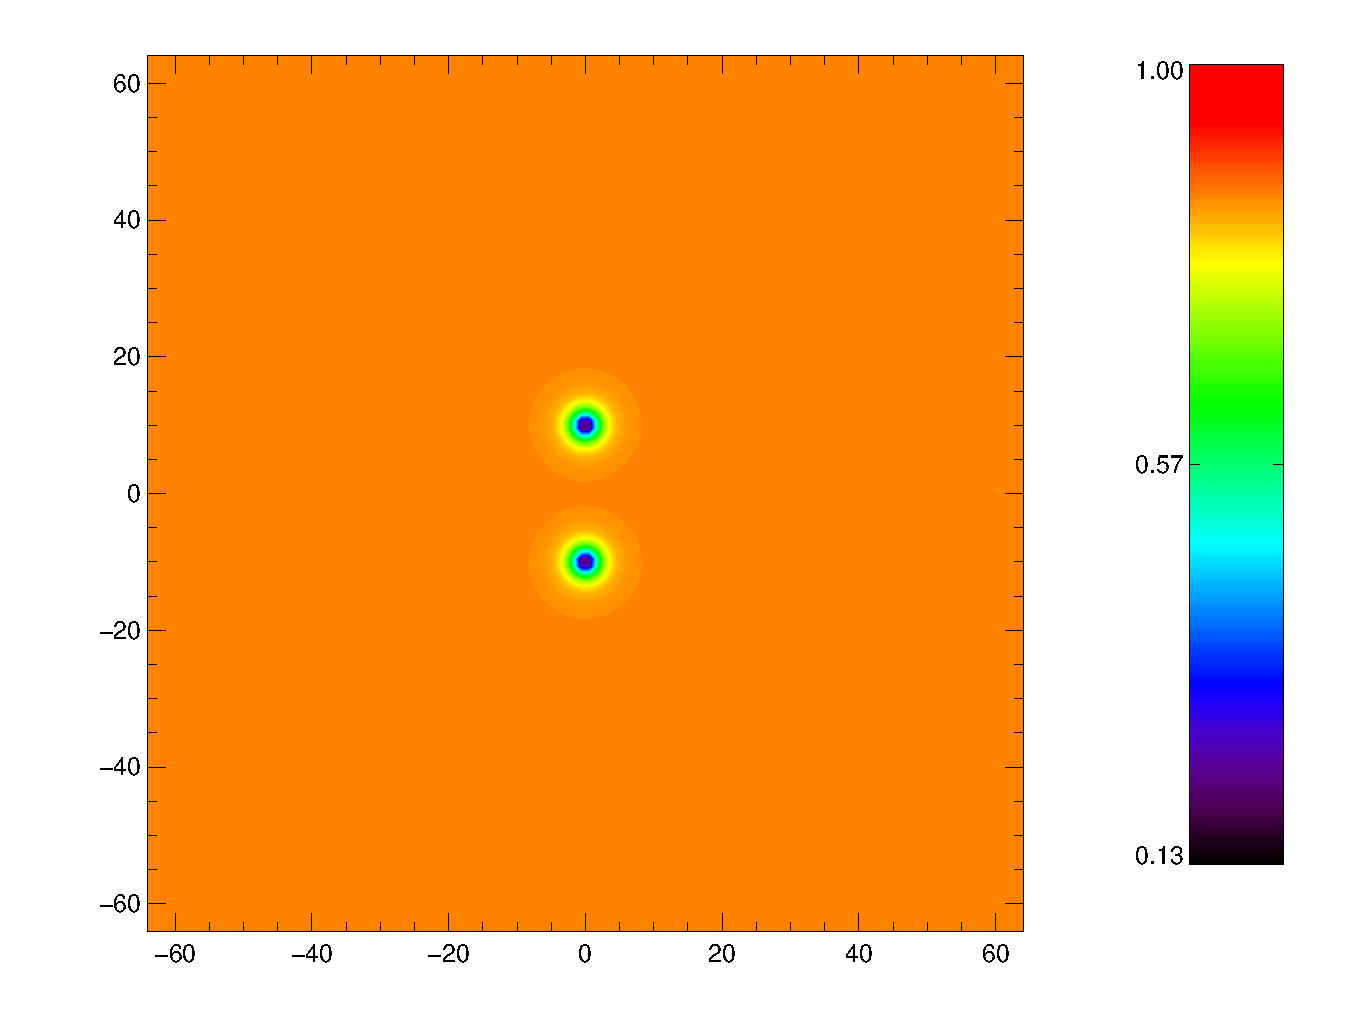
\includegraphics[scale=0.5]{fig/ring_ic_con}
    \caption{\label{fig:ring_ic_con}Contour plot of the density of a vortex
      ring of radius $R_{0}=10$ in the $(x,y)$-plane at $z=0$.}
  \end{figure}
  %
  The word \gpevar{gpe} represents an IDL program, which takes two non-optional
  arguments.  The first is the index corresponding to the first file you want
  to plot, and the second is the index corresponding to the last file you want
  to plot.  \emph{Important: For output to the screen these numbers should
  always be the same.}

  The numbers refer to the files within the \gpefile{proc} directories.  If you
  look in \gpefile{proc00}, for example, you will see a number of files named
  \gpefile{dens*******.dat}.  The arguments to \gpevar{gpe} are the numbers
  within the filenames, excluding the leading zeroes.

  So, \gpevar{gpe, 0, 0} plots \gpefile{dens0000000.dat}; \gpevar{gpe, 334,
  334} plots \gpefile{dens0000331.dat}, etc.

  The remaining arguments are optional.  The first, \gpevar{/dbl}, denotes that
  the binary data are double-precision.  You must always provide this switch
  when you have performed a double-precision run.  In a single-precision run,
  this switch is not necessary.

  The second, \gpevar{/cntr}, is a switch which turns on contour output, rather
  than the default, which is an isosurface (see
  section~\ref{subsec:isosurface_plots}).

  To quit IDL at any time type \verb"exit".

  \subsection{\label{subsec:isosurface_plots}Isosurface plots}
  Start IDL again, and do exactly as in section~\ref{subsec:contour_plots}, but
  this time leave off the \gpevar"/cntr" switch.
  
  You should see an isosurface plot in a window similar to that in
  figure~\ref{fig:ring_ic_iso}, and a control panel with various buttons on it.
  Most of the control panel buttons can be ignored.  The \verb"bbox",
  \verb"content", and \verb"axis" buttons turn on or off the bounding box, the
  content, and the axes labels respectively.  You will need to click the
  \verb"Redraw" button if you make any changes.
  %
  \begin{figure}
    \centering
    
\includegraphics[scale=1]{fig/ring_ic_iso}
    \caption{\label{fig:ring_ic_iso}Isosurface plot of the density of a vortex
      ring of radius $R_{0}=10$ at the level $\abs{\psi}^{2} = 0.75$.}
  \end{figure}
  %
  Left-click and hold in the white window and you can move the view around;
  right-clicking zooms in and out, and middle-clicking moves the centre
  viewpoint.  Depending on the speed of your machine, and the complexity of the
  displayed image, zooming and moving the view might be a little slow, so move
  the mouse slowly, and avoid large jerky movements.

  The coloured bar in the control panel is a histogram of the density, and
  clicking in here will redraw the isosurface at the new density level, which
  is shown toward the right-hand side of the control panel.

  Pressing \verb"auto" will automatically redraw the isosurface when other
  boxes are checked, for example, the axes, or whether the surface is solid,
  wireframe, or a series of points.  If the display is too slow, selecting
  \verb"points" or \verb"wireframe" instead of \verb"solid" will speed it up.

  \subsection{Animations}
  By saving a series of snapshots of 2D or 3D data it is possible to then
  combine them into an animation.

  From the run directory run the script \gpefile{create-links}.  This will
  create a directory \gpefile{links}, which contains renamed symbolic links
  (shortcuts) pointing to the isosurface files within each process directory.
  This is to make sure that the files are numbered sequentially in steps of
  one.  The \gpefile{create-links} script is located in the \gpefile{scripts}
  subdirectory of the main code directory.  Giving it the argument
  \gpefile{--help} will provide usage instructions.

  \subsubsection{Contour animations}
  Change to the links directory and create another directory called
  \gpefile{images}, then start IDL again.

  Now type
  %
  \begin{Verbatim}
    gpe, 0, 9, /dbl, /cntr, /c_anim
  \end{Verbatim}
  %
  This will loop over all data files numbered 0 to 9 and save
  \verb"con_dens*******.png" files in the \gpefile{images} directory.  (If you
  left the \gpeexample{ring} example parameters at their defaults, then you
  should actually find 100 data files in each \gpefile{proc} directory, so you
  could do plots from 0 to 99 if you wish.)

  \emph{If you miss off the /c\_anim switch here, you will get all the
  plots shown to the screen.  When you are plotting 100 or more files, this
  can be very bad and in some cases might run your machine out of memory.}

  Now change to the \verb"images" directory and run the \gpefile{makemovie}
  script, which is located in the \gpefile{scripts} subdirectory of the main
  code directory:
  %
  \begin{Verbatim}
    makemovie -i png -p con_dens
  \end{Verbatim}
  %
  which will create an AVI animation out of the PNG files, with 10 frames,
  saving the output as \gpefile{output.avi}.

  You can then play the animation with any media player, for example,
  %
  \begin{Verbatim}
    mplayer output.avi
  \end{Verbatim}
  %
  The animation is very short; if it works you can try a longer animation by
  repeating the \gpevar{gpe} IDL command with arguments 0 and 99.

  \subsubsection{Isosurface animations}
  Rename the \gpefile{images} directory to something else, and recreate an
  empty \gpefile{images} directory.  Start IDL and this time type
  %
  \begin{Verbatim}
    gpe, 0, 9, /png
  \end{Verbatim}
  %
  As for the contour plots before, this will save PNG files in the
  \gpefile{images} directory, which you can then convert into an animation
  using \gpefile{makemovie}.

  \emph{If you miss off the /png switch, all the output will again go to the
  screen.  This should be avoided if possible.}

  \section{\label{sec:restart}Restarting the code}
  After a run, you might decide that you would like to restart the code from
  where you left off, for example, maybe you started your run in imaginary
  time, and now want to switch to real time, or maybe you did not run for quite
  long enough.

  If this is the case, create a new directory where the restarted run will take
  place, and copy \gpefile{parameters.in}, \gpefile{ic.in}, \gpefile{run.in},
  \gpefile{run.sh}, and the executable \gpefile{gpe} from the initial run
  directory to the restart directory.

  Now edit \gpefile{run.in}, change \gpevar{restart} to \gpevar{.true.}, and
  make any other changes necessary.  Recompilation is not needed when making
  changes only to \gpefile{run.in}.

  Now type
  %
  \begin{Verbatim}
    ./run.sh -r <initial run directory> <nprocs>
  \end{Verbatim}
  %
  where \verb"<initial run directory>" is the directory of the run which you
  want to continue.  This will copy the \gpefile{end\_state.dat} files from the
  \gpefile{proc} directories to the restart directory (suitably renamed).  The
  \gpefile{log.txt} file should then report that the code is
  %
  \begin{Verbatim}
    Getting restart conditions
  \end{Verbatim}
  %
  and will restart from where it left off.
\end{chapter}
